% =============================================================================
%  Section 3 -- Experimentation & Results
% =============================================================================

\section{Experimentation \& Results}

% --- Section divider --------------------------------------------------------
\sectiondivider{Experimentation \& Results}{Five experiments, two sensitivity sweeps, one headline finding}{sec:experiments}

% --- Subsection: LSTM Progression ------------------------------------------
\subsection{LSTM Evolution}

\begin{frame}{LSTM evolution: Stage 01 $\rightarrow$ Stage 02 $\rightarrow$ Stage 03}
\hypertarget{sub:evolution}{}%
\setlength{\tabcolsep}{3pt}
\renewcommand{\arraystretch}{0.95}
\footnotesize
\begin{center}
\textbf{Table 4.} \itshape BiLSTM stage progression on 80/20 stratified split (seed 42).\\[1pt]
\upshape
\begin{tabular}{l c c c}
\toprule
 & \textbf{Stage 01} & \textbf{Stage 02} & \textbf{Stage 03 (final)} \\
\midrule
\textbf{Dataset}        & 280 clips, 5 players & 484 clips, 6 players & 484 clips, 6 players \\
\textbf{Output classes} & 10 (raw grades)      & 5 (grouped)          & 5 (grouped) \\
\textbf{Joints / feats} & 3 / 6                & 4 / 8                & 4 / 8 \\
\textbf{Interpolation}  & --                   & linear               & linear \\
\textbf{Class weights}  & --                   & balanced             & balanced \\
\textbf{Hidden units}\textsuperscript{*}   & 128 / 64             & 128 / 64             & \alert{64 / 32} \\
\textbf{Regularization} & --                   & --                   & L2 ($10^{-4}$), dropout 0.40/0.35 \\
\textbf{Augmentation}   & --                   & --                   & Gaussian noise $\sigma\!=\!0.02$, $\times 2$ \\
\midrule
\textbf{Accuracy}       & 16.1\%               & 24.7\%               & \textbf{29.9\%} \\
\textbf{Macro F1}       & 0.09                 & 0.23                 & 0.23 \\
\bottomrule
\end{tabular}\\[2pt]
{\scriptsize\itshape \textsuperscript{*}All three stages use a \alert{2-layer stacked Bidirectional LSTM}; only the hidden-unit sizes per layer change.}
\end{center}
\vspace{2pt}
\begin{infoBox}\scriptsize
\textbf{Largest gain: $+8.6$ pp} came from \alert{pipeline changes} (5-class, interpolation, class weights), not from architecture. \textbf{\color{tecdark}Stage 03 is the documented final BiLSTM}; two sensitivity analyses push it further (next slides).
\end{infoBox}
\end{frame}

% --- Stage progression frame removed: redundant with the Table-3 frame above.
%     The diagnostic narrative (why each stage's interventions, what pain
%     each one fixed) is preserved in others/QA_BANK.md and the deep dive
%     for Q&A preparation, but does not need its own slide.

% --- Subsection: Model Comparison ------------------------------------------
\subsection{Model Comparison}

\begin{frame}{Comparison of three temporal models}
\hypertarget{sub:comparison}{}%
\setlength{\tabcolsep}{6pt}
\small
\begin{center}
\textbf{Table 5.} \itshape Head-to-head comparison of the three temporal architectures (80/20 split, seed 42).\\[2pt]
\upshape
\begin{tabular}{l c c c}
\toprule
\textbf{Metric} & \textbf{BiLSTM (Stage 03)} & \textbf{BiGRU (Stage 01)} & \textbf{TCN (Stage 01)} \\
\midrule
Architecture           & BiLSTM 64/32 & BiGRU 64/32 & 3$\times$ 1-D conv.\ (Conv1D) \\
Test set               & 97           & 97          & 97 \\
\midrule
\textbf{Accuracy}      & \textbf{29.9\%} & 26.8\%   & \textbf{29.9\%} \\
\textbf{Macro F1}      & 0.23         & 0.21        & \textbf{0.24} \\
\textbf{Weighted F1}   & \textbf{0.30} & 0.26       & \textbf{0.30} \\
Spearman $\rho$ ($p$)  & 0.03 (0.76)  & 0.12 (0.26) & 0.14 (0.18) \\
\bottomrule
\end{tabular}
\end{center}
\vspace{4pt}
\begin{itemize}\small
    \item BiLSTM and TCN tied on accuracy; TCN slightly higher macro F1 (better on \emph{Excellent}).
    \item BiGRU trails by 3.1~pp -- merged gating loses temporal information.
    \item Severe overfitting: BiLSTM and BiGRU reach train $\sim\!100\%$, TCN plateaus at $\sim\!80\%$; test $\sim\!30\%$ for all $\Rightarrow$ data bottleneck.
\end{itemize}
\end{frame}

\begin{frame}{Stage 03 BiLSTM: confusion matrix}
\begin{columns}[T,onlytextwidth]
\begin{column}{0.55\textwidth}
\centering
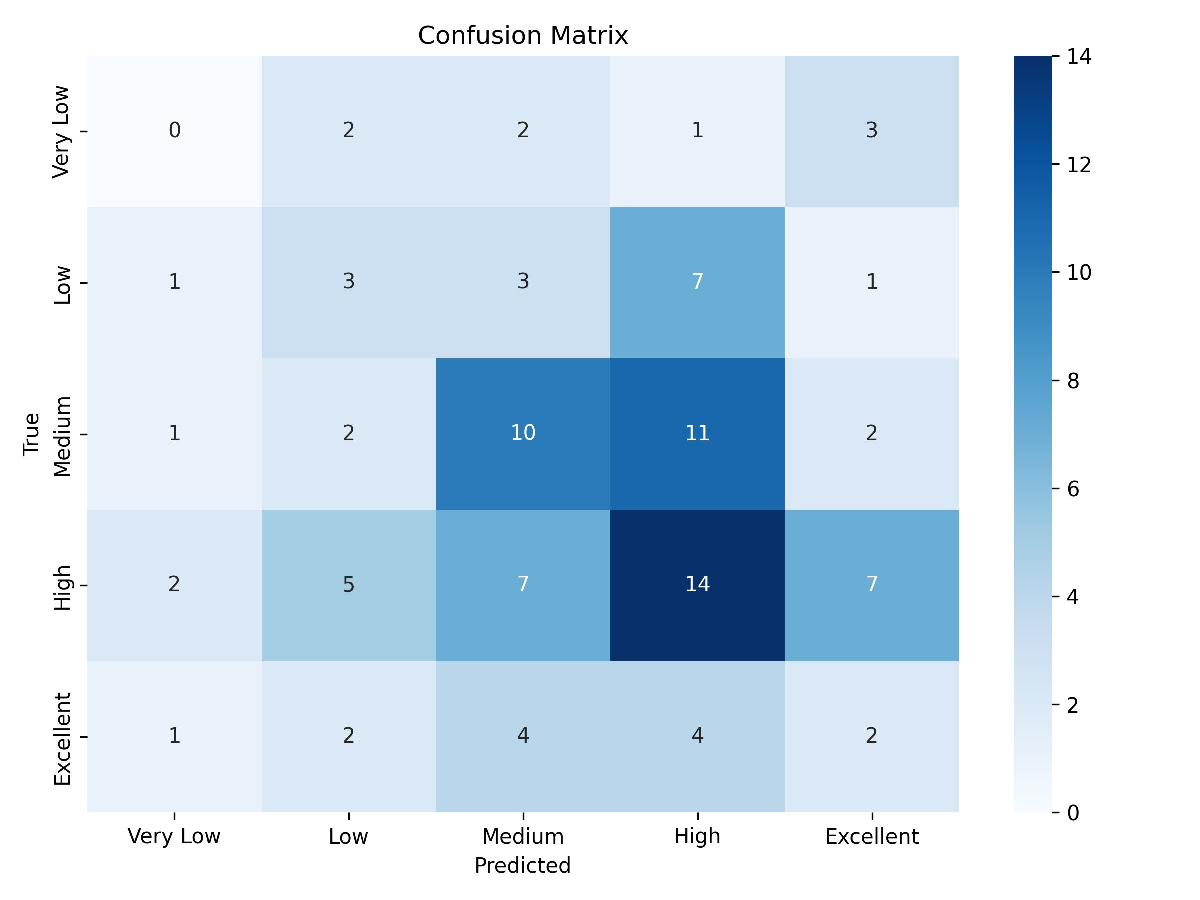
\includegraphics[width=\linewidth,height=0.72\textheight,keepaspectratio]{./DATA/images/experimentation/lstm_test03_confusion.pdf}\\[2pt]
{\scriptsize\textbf{Figure 9.} \itshape Stage 03 BiLSTM confusion matrix on the 80/20 test fold ($n\!=\!97$).}
\end{column}
\begin{column}{0.43\textwidth}\small
\textbf{\color{tecdark}Observations:}
\begin{itemize}
    \item Diagonal mass on \alert{Medium} (10/26) and \alert{High} (14/35).
    \item \emph{Very Low} (8 samples): zero recall -- spreads to Low / Medium.
    \item Off-diagonal mass on \alert{adjacent} classes $\Rightarrow$ ordinal confusion.
    \item No catastrophic Excellent$\leftrightarrow$Very Low confusion: the model has learned the gross gradient.
\end{itemize}
\end{column}
\end{columns}
\end{frame}

% --- Subsection: Sensitivity Analyses --------------------------------------
\subsection{Sensitivity Analyses}

\begin{frame}{Sensitivity 1: Loss function $\times$ Optimizer (BiLSTM)}
\hypertarget{sub:sensitivity}{}%
\begin{columns}[T,onlytextwidth]
\begin{column}{0.50\textwidth}
\setlength{\tabcolsep}{4pt}\scriptsize
\begin{center}
\textbf{Table 6.} \itshape Sensitivity 1 -- 2$\times$2 loss/optimizer grid.\\[2pt]
\upshape
\begin{tabular}{l l c c c}
\toprule
\textbf{Loss} & \textbf{Opt.} & \textbf{Acc.} & \textbf{F1$_m$} & \textbf{$\rho$ ($p$)} \\
\midrule
XEnt    & Adam (baseline) & 26.8\% & 0.21 & $-$0.02 (0.85) \\
\rowcolor{tecblue!10}
\textbf{XEnt} & \textbf{SGD}(0.9) & \textbf{35.1\%} & \textbf{0.30} & \textbf{0.19 (0.06)} \\
MSE     & Adam            & 35.1\% & 0.27 & 0.10 (0.31) \\
MSE     & SGD(0.9)        & 27.8\% & 0.23 & 0.07 (0.50) \\
\bottomrule
\end{tabular}
\end{center}
\vspace{4pt}
\textbf{\color{tecdark}Key findings:}
\begin{itemize}\scriptsize
    \item \alert{Cross-entropy (XEnt) + Stochastic Gradient Descent (SGD)}: $+8.3$~pp accuracy, $+0.09$ F1, $\rho\!=\!0.19$ ($p\!=\!0.06$) -- strongest single BiLSTM run.
    \item Adam~\cite{Adam2014} overfits faster on 484 clips; SGD's smoother updates win.
    \item Combining both changes (Mean Squared Error (MSE) + SGD) \emph{does not} stack.
\end{itemize}
\end{column}
\begin{column}{0.48\textwidth}
\centering
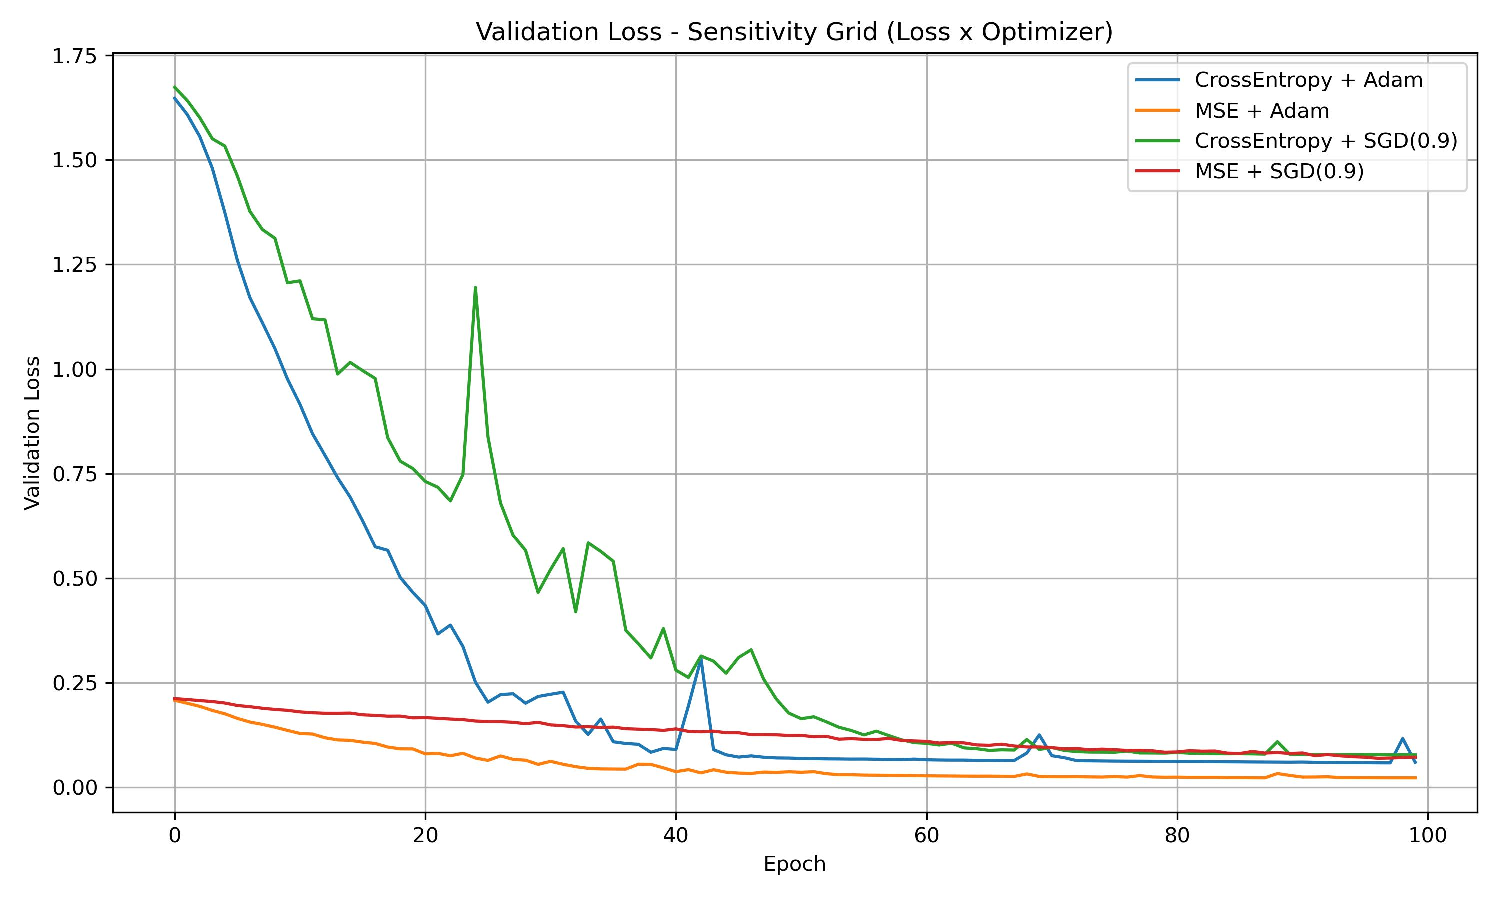
\includegraphics[width=\linewidth,height=0.7\textheight,keepaspectratio]{./DATA/images/experimentation/sensitivity_overlay.pdf}\\[2pt]
{\scriptsize\textbf{Figure 10.} \itshape Per-cell val-loss curves; MSE and XEnt sit on different numerical scales (not directly comparable). Ranking by test accuracy is in Table~6 -- winner: \alert{XEnt\,+\,SGD at 35.1\%}.}
\end{column}
\end{columns}
\end{frame}

\begin{frame}{Sensitivity 2: Train/Test split ratio (BiLSTM)}
\begin{columns}[T,onlytextwidth]
\begin{column}{0.50\textwidth}
\setlength{\tabcolsep}{4pt}\scriptsize
\begin{center}
\textbf{Table 7.} \itshape Sensitivity 2 -- 5-point train-fraction sweep.\\[2pt]
\upshape
\begin{tabular}{c c c c c}
\toprule
\textbf{Train frac.} & \textbf{Train / Test} & \textbf{Acc.} & \textbf{F1$_m$} & \textbf{$\rho$ ($p$)} \\
\midrule
0.50 & 242 / 242 & 35.5\% & 0.29 & \textbf{0.22 ($<\!0.001$)} \\
\rowcolor{tecblue!10}
\textbf{0.60} & 290 / 194 & \textbf{36.1\%} & 0.28 & \textbf{0.23 (0.001)} \\
0.70 & 338 / 146 & 34.2\% & 0.28 & 0.14 (0.09) \\
0.80\,(base)$^\dagger$ & 387 / 97 & \textbf{29.9\%} & 0.23 & 0.03 (0.76) \\
0.90 & 435 / 49  & 28.6\% & 0.24 & 0.05 (0.71) \\
\bottomrule
\end{tabular}\\[2pt]
{\tiny $^\dagger$The 0.80 row reports the documented Stage 03 final (LSTM Test03); the four other fractions come from the \texttt{runSplitAnalysis} sweep. Both share architecture, hyperparameters, and stratified split (\texttt{random\_state=42}); the $\sim$3\,pp run-to-run variance between code paths is consistent with non-explicit RNG seeding at $N\!=\!484$.}
\end{center}
\vspace{2pt}
\textbf{\color{tecdark}Counter-intuitive:}
\begin{itemize}\scriptsize
    \item Smaller training fractions \alert{win}.
    \item 0.60: \textbf{36.1\%}, $\rho\!=\!0.23$, $p\!=\!0.001$ -- the \emph{only} BiLSTM run with statistically significant $\rho$.
    \item Augmentation ($\times 2$) inflates training redundancy beyond what 100 epochs can absorb.
\end{itemize}
\end{column}
\begin{column}{0.48\textwidth}
\centering
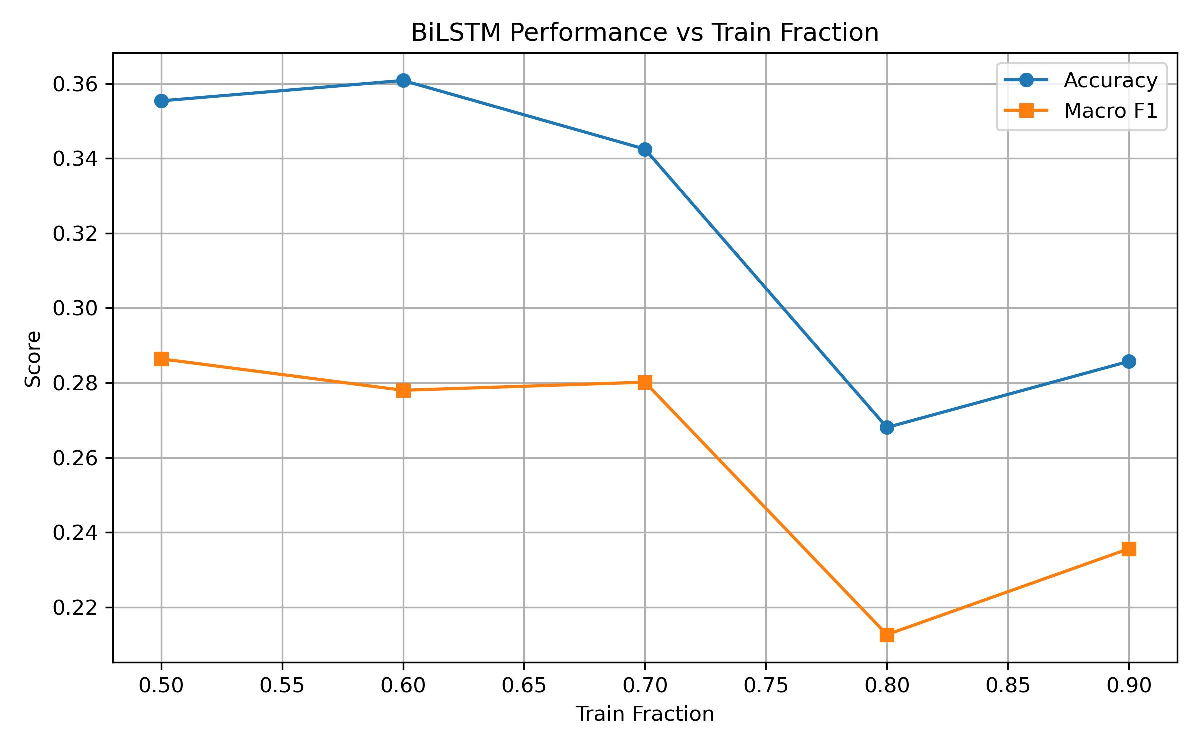
\includegraphics[width=\linewidth,height=0.7\textheight,keepaspectratio]{./DATA/images/experimentation/split_trend.pdf}\\[2pt]
{\scriptsize\textbf{Figure 11.} \itshape Accuracy and macro F1 vs.\ training fraction.}
\end{column}
\end{columns}
\end{frame}

% --- Subsection: Headline Finding ------------------------------------------
\subsection{Headline Finding}

\begin{frame}{\emph{Method is data-limited, not method-limited}}
\hypertarget{sub:headline}{}%
\begin{columns}[T,onlytextwidth]
\begin{column}{0.45\textwidth}
\centering
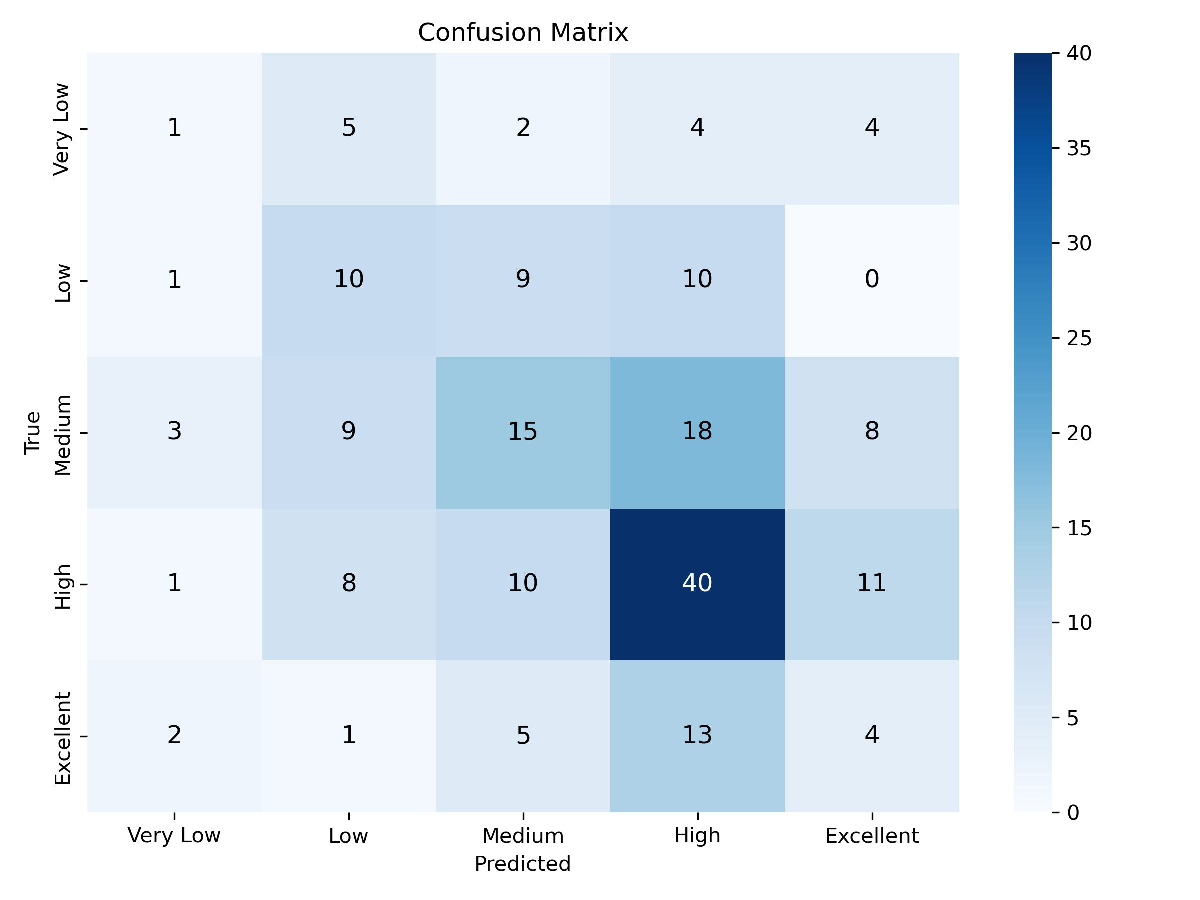
\includegraphics[width=\linewidth,height=0.66\textheight,keepaspectratio]{./DATA/images/experimentation/split_confusion_06.pdf}\\[2pt]
{\scriptsize\textbf{Figure 12.} \itshape Confusion matrix at the 60/40 split: broader coverage of minority classes.}
\end{column}
\hspace{0.02\textwidth}
\begin{column}{0.51\textwidth}
\begin{alertblock}{The $+6$ percentage-point (pp) gain -- and the $\rho$ flip}
\footnotesize Same architecture, same labels, same hyperparameters -- only the train/test fraction changed.\\[6pt]
\centerline{$29.9\%\;\Longrightarrow\;\textbf{36.1\%},\quad \rho\!:\;0.03\!\rightarrow\!\textbf{0.23},\quad p\!:\;0.76\!\rightarrow\!\textbf{0.001}$}\\[6pt]
{\scriptsize\itshape pp = percentage points: absolute difference between two percentages ($36.1-29.9=6.2$).}
\end{alertblock}
\vspace{4pt}
\begin{itemize}\scriptsize
    \item If the architecture / pipeline were the bottleneck, accuracy would be \alert{roughly flat across splits} -- ours is not.
    \item The Spearman $\rho$ \alert{crosses the conventional significance threshold} ($p\!<\!0.05$) only when the test fold is large enough -- the textbook signature of a \alert{data-limited regime}, not a methodological flaw.
\end{itemize}
\end{column}
\end{columns}
\end{frame}
